\documentclass[utf8]{psta}

\subjclass[UDC]{004.42}
\subjclass[BBC]{32.973}
\subjclass[2010]{68N19}

\usepackage{mathtools}
\usepackage{amsfonts}

\title[исследование эффективности векторизации]{Исследование эффективности векторизации гнезд циклов с нерегулярным числом итераций}    

\author{Рыбаков, Алексей Анатольевич}
\address{Межведомственный суперкомпьютерный центр Российской академии наук -- филиал Федерального государственного учреждения <<Федеральный научный центр Научно-исследовательский институт системных исследований Российской академии наук>> (МСЦ РАН -- филиал ФГУ ФНЦ НИИСИ РАН)}
\email{rybakov@jscc.ru}

\info{Рыбаков Алексей Анатольевич -- к ф.-м. н., внс МСЦ РАН --
филиала ФГУ ФНЦ НИИСИ РАН. Области научных интересов
-- математическое моделирование задач газовой динамики с
использованием суперкомпьютеров, методы построения и
управления расчетными сетками, дискретная математика,
теория графов, модели случайных графов, параллельное
программирование, функциональное программирование.}
\image{pics/Rybakov_photo}
\orcid{0000-0002-9755-8830}    

\author{Шумилин, Сергей Сергеевич}
\address{Межведомственный суперкомпьютерный центр Российской академии наук -- филиал Федерального государственного учреждения <<Федеральный научный центр Научно-исследовательский институт системных исследований Российской академии наук>> (МСЦ РАН -- филиал ФГУ ФНЦ НИИСИ РАН)}
\email{shumilin@jscc.ru}
\info{Шумилин Сергей Сергеевич, старший инженер МСЦ РАН -- филиала ФГУ ФНЦ НИИСИ РАН. Область научных интересов: машинное обучение, анализ данных, алгоритмы, параллельное программирование.}
\image{pics/Shumilin_photo}
\orcid{0000-0002-3953-7054}    

\keywords{векторизация, AVX-512, гнезда циклов с нерегулярным числом итераций, сортировка Шелла, теоретическое ускорение}
\begin{abstract}
Векторизация вычислений является важной низкоуровневой оптимизацией, используемой для создания высокоэффективного параллельного кода. 
Однако, при использовании ее в контексте с неизвестным профилем исполнения существует опасность низкой эффективности применения. 
Особенно ярко это проявляется при векторизации гнезд циклов с нерегулярным числом итераций внутреннего цикла. 
В статье рассматривается сравнение теоретической и практической эффективности векторизации на примере сортировки Шелла, так как данный программный код является крайне неудобным с точки зрения применения векторизации.
\end{abstract}

% Все метаданные должны также присутствовать на английском языке, 

% заключённые в  \selectlanguage{english}...,\selectlanguage{russian}: 

\selectlanguage{english} 
% All the same in English 
\title[Study of the vectorization efficiency]{Study of the vectorization efficiency of loop nests with an irregular number of iterations}
% Last name, coma other names 
\author{Rybakov,A. A.}
% Organisation, where the work done
\address{Joint Supercomputer Center of the Russian Academy of Sciences -- branch of Scientific Research Institute of System Analysis of the Russian Academy of Sciences, Leninsky prospect 32a, Moscow, 119334, Russia}
% author email
\email{rybakov.aax@gmail.com}
% support notes

\author{Shumilin,S. S.}
\email{shumilin@jscc.ru}

% Other information about author only on paper language 
%\info{} %
% author photo
%\image{}
%\orcid{}
% Repeat the same fore each of other authors
%
\begin{abstract}
Computation vectorization is an important low-level optimization used to create highly efficient parallel code.
However, when used in context with an unknown program execution profile, a danger of low effectiveness of the application emerges.
This is especially pronounced when vectorizing nests of cycles with an irregular number of iterations of the inner loop.
The article discusses a comparison of the theoretical and practical efficiency of vectorization on the example of Shell sorting, since this program code is extremely inconvenient for vectorization.
\end{abstract}
\selectlanguage{russian} % Не забывайте отметить возврат на русский язык
% Для локального переключения на другой язык используйте команду 
% \foreignlanguage{english}{Text in English}

\begin{document}           
\maketitle   

\section*{Введение}

В данной статье векторизация рассматривается применительно к набору инструкций AVX-512, представляющих собой 512-битное расширение 256-битных AVX инструкций из набора команд Intel x86 \cite{intel_manual}, поддержанное в семействах микропроцессоров Intel Xeon Phi KNL \cite{Jeffers} и Intel Xeon Skylake. 
Данный набор состоит из следующих подмножеств: AVX-512F (Foundation) -- основной набор векторных инструкций с поддержкой маскирования, AVX-512PF (PreFetch) -- инструкции предварительной подкачки данных из памяти, AVX-512ER (Exponential and Reciprocal) -- команды для вычисления экспоненты и обратных значений, AVX-512CD (Conflict Detection) -- инструкции для определения конфликтов, AVX-512BW и AVX-512DQ, поддержанные в Skylake. 
В следующих поколениях процессоров набор инструкций AVX-512 расширяется еще больше, в него входят команды для работы с 52-битными целочисленными значениями, специальные команды для работы с нейросетями и AES шифрованием, реализация арифметики полей Галуа, имплементация специальных битовых операций, а также новый класс комбинированных операций.

Использование масок в векторных операциях, позволяющих осуществлять выборочную обработку отдельных элементов векторов, позволяет реализовать предикатный режим исполнения операций. 
В совокупности с многообразием операций перестановки элементов векторов, комбинированными операциями, операциями множественного доступа в память по произвольным адресам, и многими другими особенностями набора инструкций AVX-512 это позволяет создавать качественный параллельный код, приводящий к кратному ускорению.

Для упрощения векторизации исходного кода для компилятора icc доступны специальные функции-интринсики \cite{compiler_guide, intrinsic_guide}, являющиеся обертками к инструкциям или группам инструкций AVX-512. 
Использование функций-интринсиков и встроенных типов данных для поддержки 512-битных векторов позволяет создавать конкретные векторные инструкции в результирующем коде, оперируя при этом высокоуровневыми сущностями языка программирования C. 
Из множества интринсиков можно выделить следующие группы функций, схожие по структуре. Функции \texttt{swizzle}, \texttt{shuffle}, \texttt{permute} и \texttt{permutevar} осуществляют перестановку элементов вектора и раскрываются в последовательность операций, в которой присутвует операция \texttt{shuf} и пересылка по маске. Для большего числа операций AVX"~512 реализованы соответствующие инстринсики, раскрывающиеся в одну конкретную операцию. 
Среди них арифметические операции, побитовые операции, операции чтения из памяти и записи в память, операции конвертации, слияние двух векторов, нахождение обратных значений, получение минимума и максимума из двух значений, операции сравнения, операции с масками, комбинированные операции и другие. 
Некоторые инстринсики, особенно предназначенные для выполнения упакованных трансцендентных операций, раскрываются просто в вызов библиотечной функции (например \texttt{log}, \texttt{hypot}, тригонометрические функции).

В качестве объекта исследования для данной статьи была выбрана сортировка Шелла, обладающая крайне неудобным контекстом исполнения для векторизации с помощью инструкций AVX-512. 

\section{Описание сортировки Шелла}

Сортировка Шелла \cite{Knuth} представляет собой расширение сортировки вставками, которое работает быстрее, так как позволяет на ранних этапах упорядочить далеко расположенные друг от друга элементы массива, это приводит к тому, что массив становится частично упорядоченным. 
Во время сортировки Шелла выполняется последовательная сортировка подмассивов основного массива, являющихся срезами, при этом шаг среза постоянно уменьшается и на завершающем этапе выполняется обычная сортировка вставками (это соответствует срезу массива с шагом 1).
Выполнение сортировки срезов массива с большими шагами облегчает сортировку срезов с меньшими значениями шага, эффективность сортировки существенно зависит от выбранной последовательности шагов. 
В литературе описано множество существующих последовательностей, из которых мы будем анализировать лишь следующие, представленные в Табл.~\ref{tab:shell_sequences}:

\renewcommand{\arraystretch}{1.8}
\renewcommand{\tabcolsep}{4.0}
\begin{table}[H]
\caption{\label{tab:shell_sequences}Различные последовательности шагов, используемые в сортировке Шелла}
\begin{center}

\begin{tabular}{| c | c |}
\hline
\bf{Последовательность} & \bf{Формула} \\
\hline
Последовательность Шелла, 1959 г. &
$k_1 = \lfloor \frac{N}{2} \rfloor, k_i = \lfloor \frac{k_{i - 1}}{2} \rfloor, k_t = 1$ \\
\hline
Последовательность Хиббарда, 1963 г. &
$2^i - 1 \le N, i \in \mathbb{N}$ \\
\hline
Последовательность Пратта, 1971 г. &
$2^i \cdot 3^j \le \frac{N}{2}, i \in \mathbb{N}, j \in \mathbb{N}$ \\
\hline
Последовательность Седжвика, 1986 г. &
$k_i = 
\begin{cases}
  9 \cdot 2^i - 9 \cdot 2^{\frac{i}{2}} + 1, k \ even\\
  8 \cdot 2^i - 6 \cdot 2^{\frac{i + 1}{2}} + 1, k \ odd
\end{cases}$ \\
\hline
\end{tabular}
\end{center}
\end{table} 

Каноническая реализация сортировки Шелла состоит из гнезда циклов, содержащего три цикла. 
Внешний цикл выполняется по всем шагам из используемой последовательности шагов, начиная с максимального и заканчивая единицей. 
Два внутренних цикла осуществляют сортировку всех подмассивов, являющихся срезами исходного массива с текущим шагом $k$ (Рис.~\ref{pic:shell_code}).

\begin{figure}
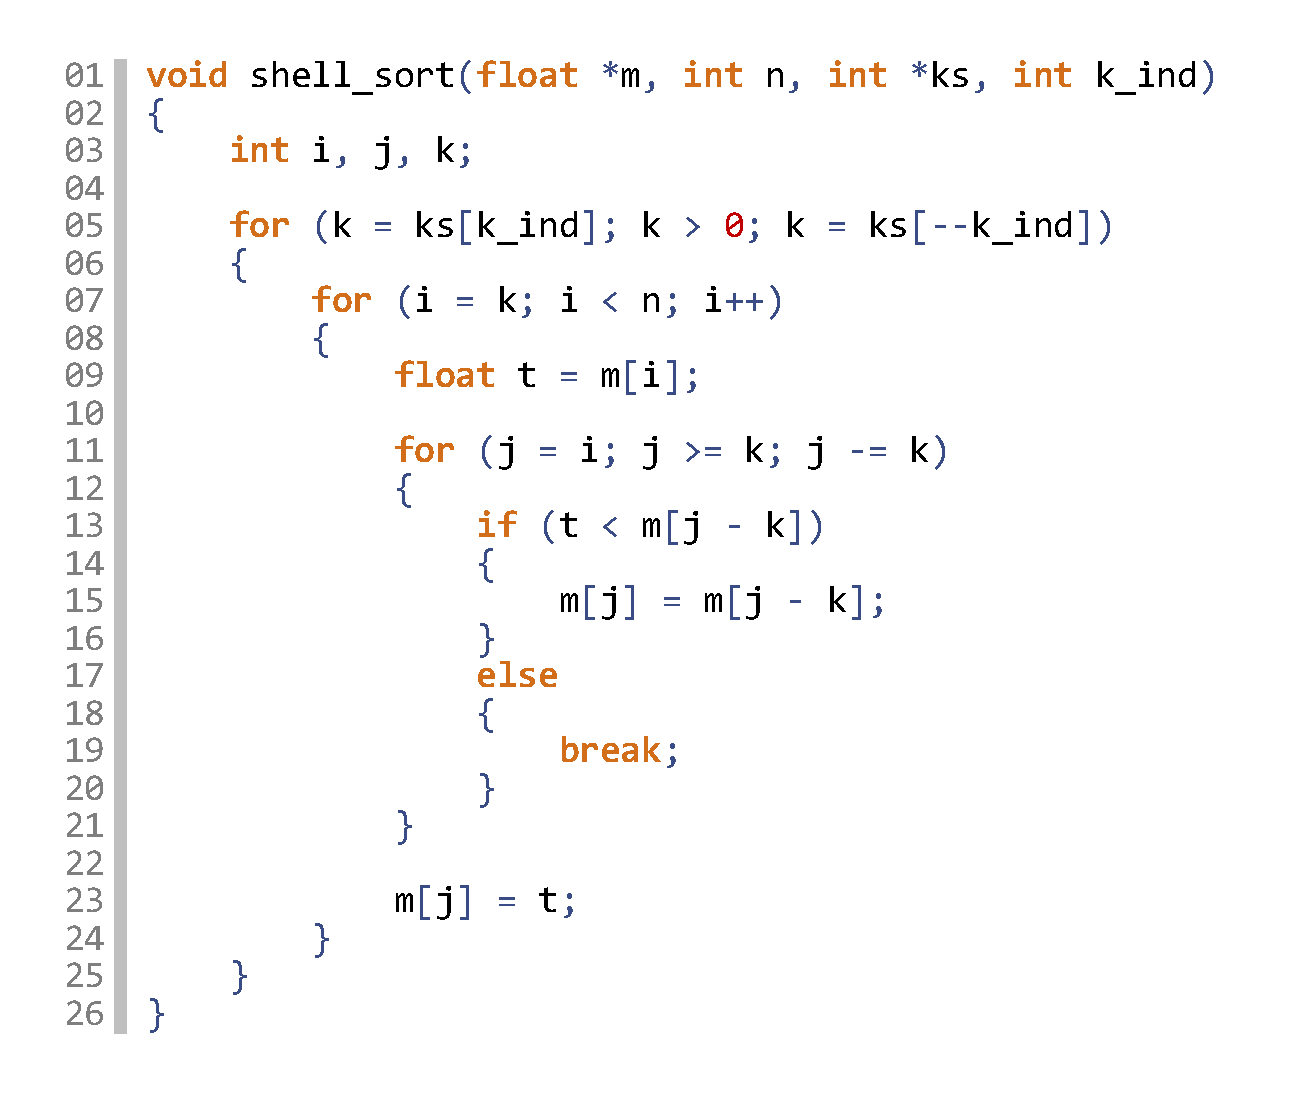
\includegraphics[width=8cm]{pics/pic_shell_code}
\caption{Реализация сортировки Шелла для произвольной последовательности шагов}
\label{pic:shell_code}
\end{figure}

\section{Векторизация сортировки Шелла с помощью инструкций AVX-512}

Рассмотрим возможности по векторизации сортировки Шелла для массива вещественных значений типа \texttt{float} (вектор AVX-512 содержит 16 таких значений). 
Самый вложенный цикл (цикл с счетчиком $j$, будем называть его просто внутренним) выполняет сортировку одного среза, состоящего из элементов массива, с расстоянием $k$ между соседними элементами.
Внутренний цикл не может быть векторизован без выполнения дополнительных модификаций кода, так как между записью элемента $m[j]$ и чтением элемента $m[j - k]$ существует межитерационная зависимость. 
Однако, можно заметить, что две итерации среднего по вложенности цикла (цикла с индуктивной переменной $i$, будем называть его промежуточным) с номерами $i_1$ и $i_2$ не пересекаются по данным и могут быть выполнены параллельно при выполнении условия $|i_1 - i_2| < k$. 
Выполним декомпозицию сортировки Шелла для того, чтобы можно было явно выделить ядро, поддающееся векторизации.

\begin{figure}
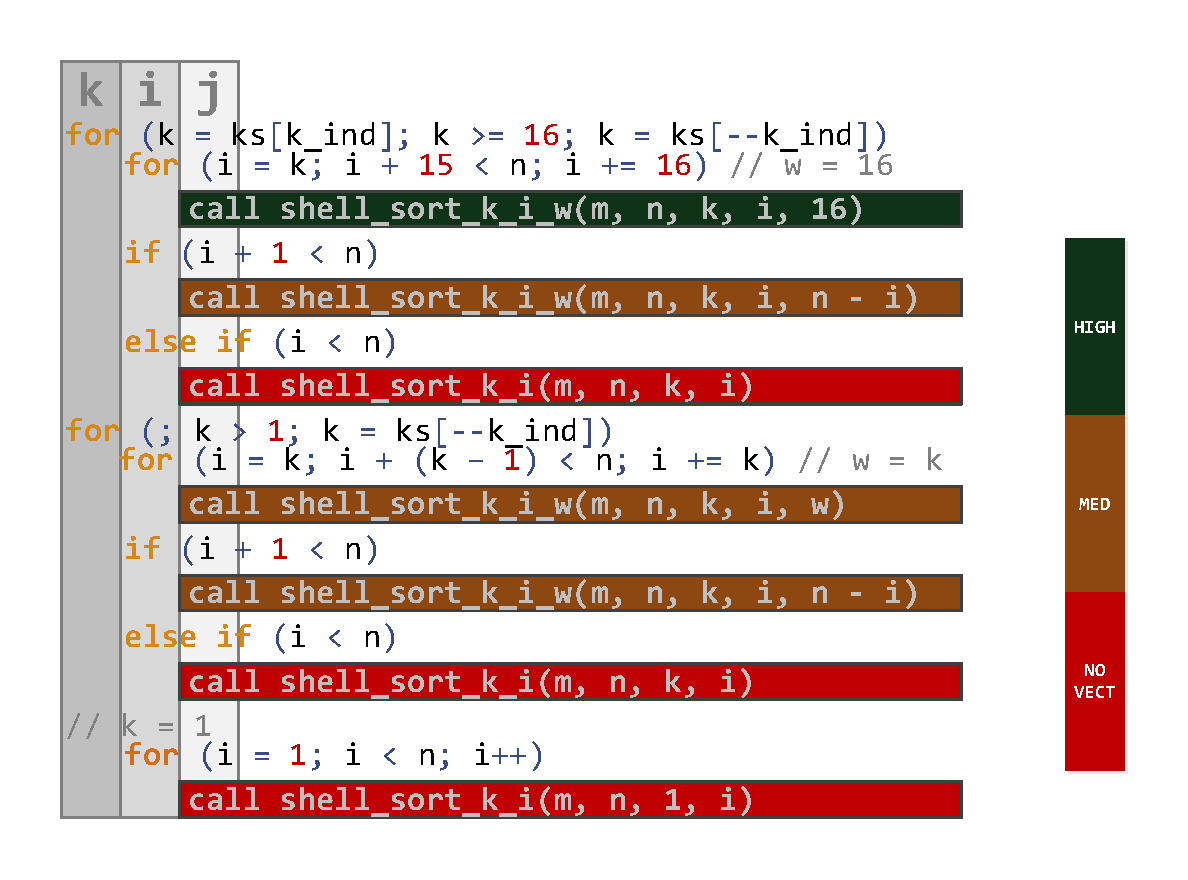
\includegraphics[width=10cm]{pics/pic_decomposition}
\caption{Декомпозиция сортировки Шелла для выделения векторизуемых участков кода}
\label{pic:decomposition}
\end{figure}

На Рис.~\ref{pic:decomposition} представлена схема декомпозиции алгоритма сортировки Шелла, в котором явно выделены участки с разной шириной векторизации. 
Сначала выделен блок для шагов $k \ge 16$. 
Для данных значений шагов можно параллельно выполнять 16 соседних итераций промежуточного цикла, при этом достигается максимальная плотность векторизации (показано зеленым цветом на схеме). 
Все итерации промежуточного цикла разбиваются на группы по 16 соседних итераций и остаток, который векторизуется с шириной меньше 16 (показано желтым цветом, а в том случае, когда остаток состоит всего из одной итерации, то векторизация не требуется, что показано красным цветом на схеме). Далее рассматривается блок значений шагов $1 < k < 16$. 
При данных значениях ширина векторизации всегда меньше 16, к тому же, как и в предыдущем блоке, возможно появление невекторизуемого остатка. 
В последнюю очередь рассматривается невекторизуемая финальная сортировка вставками для $k = 1$. 
Наличие участков кода с шириной векторизации менее 16 приводит к неоптимальному результирующему коду, однако есть более опасная причина низкой эффективности векторизации.

\begin{figure}
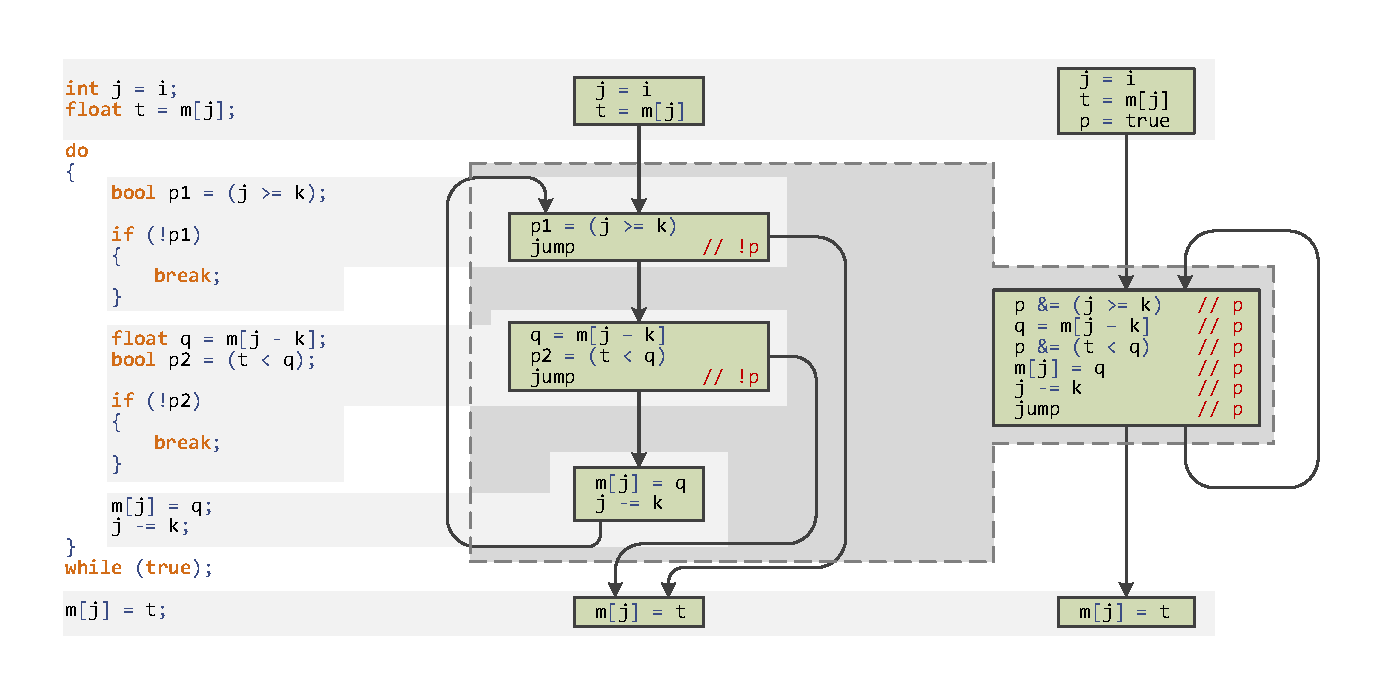
\includegraphics[width=11cm]{pics/pic_shell_cfg}
\caption{Схема перевода тела внутреннего цикла сортировки Шелла в предикатную форму}
\label{pic:shell_cfg}
\end{figure}

Функция \texttt{shell\_sort\_k\_i\_w}, появившаяся после декомпозиции алгоритма сортировки Шелла, содержит реализацию сортировки $w$ соседних срезов массива, взятых с шагом $k$. 
При этом количество итераций внутреннего цикла данной функции является неизвестным. 
Более того, количество итераций внутреннего цикла при сортировке одного среза никак не связано с количеством итераций внутреннего цикла при сортировке соседнего среза. 
Это является существенной проблемой при попытке объединить код сортировки соседних срезов, используя векторные инструкции. 
Для такого объединения необходимо переписать код сортировки среза в предикатной форме \cite{Volkonskyi}, после чего заменить все инструкции векторными аналогами, а предикаты -- векторными масками (Рис.~\ref{pic:shell_cfg}). 
При этом если до векторизации внутренний цикл завершал работу при обращении предиката в \texttt{false}, то после векторизации внутренний цикл завершит работу только если все элементы соответствующей векторной маски обнулятся. 
Таким образом, количество итераций векторизованного внутреннего цикла равно максимальному количеству итераций всех объединяемых $w$ циклов. 
Если значения количества итераций соседних объединяемых циклов различаются сильно (а для сортировки Шелла это утверждение верно), то мы получаем потерю эффективности векторизации из за низкой плотнойти масок векторных инструкций (то есть малый процент элементов векторов на самом деле обрабатывается при выполнении векторной операции).

\begin{figure}
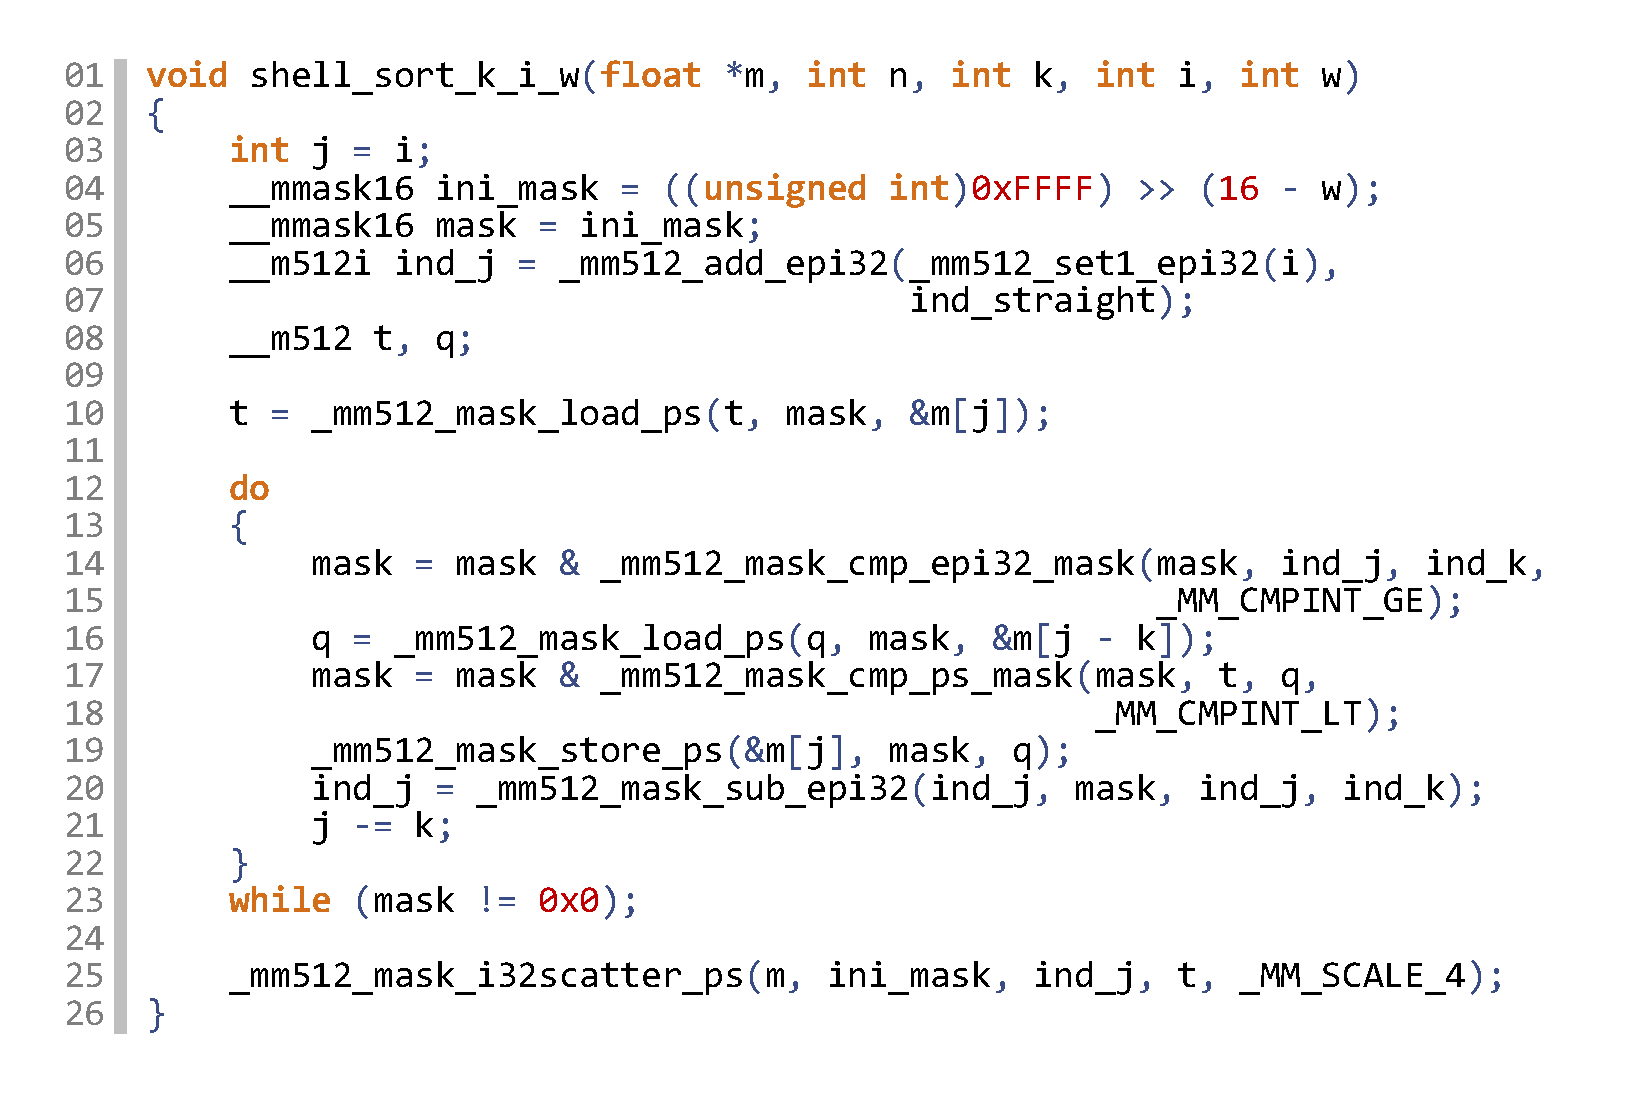
\includegraphics[width=10cm]{pics/pic_shell_code_vect}
\caption{Векторизованный вариант ядра сортировки Шелла}
\label{pic:shell_code_vect}
\end{figure}

Векторизованная версия ядра сортировки Шелла представлена на Рис.~\ref{pic:shell_code_vect}. 
Также стоит обратить внимание на появившуюся в векторном коде операцию \texttt{scatter} (Рис.~\ref{pic:shell_code_vect}, строка 25) множественной записи данных в память с произвольными смещениями относительно базового адреса. 
Данная команда появилась как векторный аналог операции записи в память из оригинального кода (Рис.~\ref{pic:shell_code}, строка 23) ввиду той же причины - нерегулярности количества итераций внутреннего цикла. 
Стоит отметить, что команды \texttt{scatter} являются крайне медленными, что также является причиной снижения эффективности векторизации.

Кроме обозначенной команды \texttt{scatter} в векторизованнос коде присутствуют другие команды обращения в память (Рис.~\ref{pic:shell_code_vect}, строки 10, 16, 19). 
Это обычные команды \texttt{load} и \texttt{store}, которые, вообще говоря, должны обращаться по выровненным адресам в памяти. 
В общем случае подаваемые им адреса конечно не являются выровненными, однако использование вместо них невыровненных обращений существенно замедляет код, поэтому было решено оставить эти инструкции.

\section{Вычисление теоретического ускорения}

В данном разделе произведем вычисление теоретического ускорения, которое может быть достигнуто при векторизации сортировки Шелла предложенным в этой статье способом. 
При этом под теоретическим ускорением будем подразумевать просто отношение количества итераций внутреннего цикла невекторизованной версии к количеству итераций внутреннего цикла в оптимизированной векторизованной версии кода. Определим данное ускорение более формально.

Сначала рассмотрим невекторизованный код. Обозначим через $T(k, i)$ количество итераций внутреннего цикла при фиксированных $k$ и $i$. 
Тогда не составляет труда вычислить общее количество итераций внутреннего цикла при выполнении сортировки (обозначим эту велечину через $T$).

\begin{equation}
T = \sum_{k \in ks}{\sum_{i = k}^{n - 1}{I(k, i)}}
\end{equation}

Теперь рассмотрим векторизованную версию кода. 
Аналогично обозначим через $T_v(k,i)$ количество итераций внутреннего цикла при фиксированных $k$ и $i$. 
Нам известно, что ширина векторизации не может превышать $k$ (из-за зависимостей по обращению к массиву), и 16 (размер вектора), то есть $w(k) = \min(k, 16)$. 
При этом весь диапазон значений $i$ от $k$ до $n - 1$, длина которого равна $n - k$ разбивается на $\lfloor \frac{n - k}{w(k)} \rfloor$ групп по $w$ элементов в каждой, и количество итераций в векторизованном цикле, соответствующем каждой группе равно максимальному значению из количеств итераций невекторизованных циклов, объединяемых в данный векторизованный цикл. 
С учетом векторизации хвостовой части цикла, получим следующую формулу для общего количества итераций векторизованного внутреннего цикла.

\begin{equation}
T_v = \sum_{k \in ks}
{
\left(
\left(
\sum_{g = 0}^{G(k) - 1}{\max_{i = k + w(k)g}^{k + w(k)(g + 1) - 1}{I(k, i)}}
\right)
+ \max_{i = k + w(k)G(k)}^{n - 1}{I(k, i)}
\right)
}
\end{equation}

где $w(k) = \min(k, 16)$, $G(k) = \lfloor \frac{n - k}{w(k)} \rfloor$. 
Значения $T = T(n)$ и $T_v = T_v(n)$ были вычислены при сортировке псевдослучайных массивов с количеством элементов от 10 тыс. до 2 млн. для каждой из последовательностей шагов Хиббарда, Пратта и Сэджвика \cite{Pratt_seq,Hib_seq,Sedjw_seq}. 
На основе этого вычислялось теоретическое ускорение $s(n) = T(n)/T_v(n)$. 
Кроме того, аналогичные характеристики рассчитывались и без учета шага $k = 1$ (данные величины обозначены $T'(n)$, $T'_v(n)$ и $s'(n)$ соответственно). 
Полученные результаты сравнивались с результатами экспериментальных запусков на микропроцессоре Intel Xeon Phi 7290 KNL.

\section{Экспериментальные результаты}
 
На Рис.~\ref{pic:acc_theor}, Рис.~\ref{pic:acc_exp} представлены результаты теоретических оценок и экспериментальных запусков, исходя из которых получены теоретическое и экспериментальное ускорение сортировки Шелла для последовательностей шагов Шелла, Хиббарда и Сэджвика. 
Из графиков видно, что даже максимальное теоретическое ускорение далеко от идеальной верхней границы (которая равна 16 для значений типа \texttt{float}), достигаемого при векторизации гнезд циклов с регулярным количеством итераций. 
Экспериментальные же результаты ожидаемо оказываются еще ниже, и в конечном итоге финальное ускорение сортировки Шелла редко превышает отметку 2.

Проанализируем гистограммы распределения количества итераций внутреннего цикла для некоторых фиксированных значений $k$. 
Из гистограмм, приведенных на Рис.~\ref{pic:shell_k_4}, Рис.~\ref{pic:shell_k_15}, Рис.~\ref{pic:hibbard_k_3}, Рис.~\ref{pic:hibbard_k_15} видно, что при переходе к векторизованной версии кода меняется характер распределения и количество выполнений внутреннего цикла с малым количеством итераций резко сокращается.

Наличие только одной итерации внутреннего цикла в невекторизованной версии кода означает, что текущий рассматриваемый элемент $m[i]$ уже стоит на своем месте в сортируемом срезе.
Для векторизованной версии одна итерация внутреннего цикла означает, что на своем месте стоят $w$ рассматриваемых элементов $w$ соседних одновременно сортируемых срезов, вероятность чего значительно ниже. 
Таким образом, итерации внутренних циклов с малым количеством итераций растворяются в векторизованном коде, что снижает его производительность.

\begin{figure}
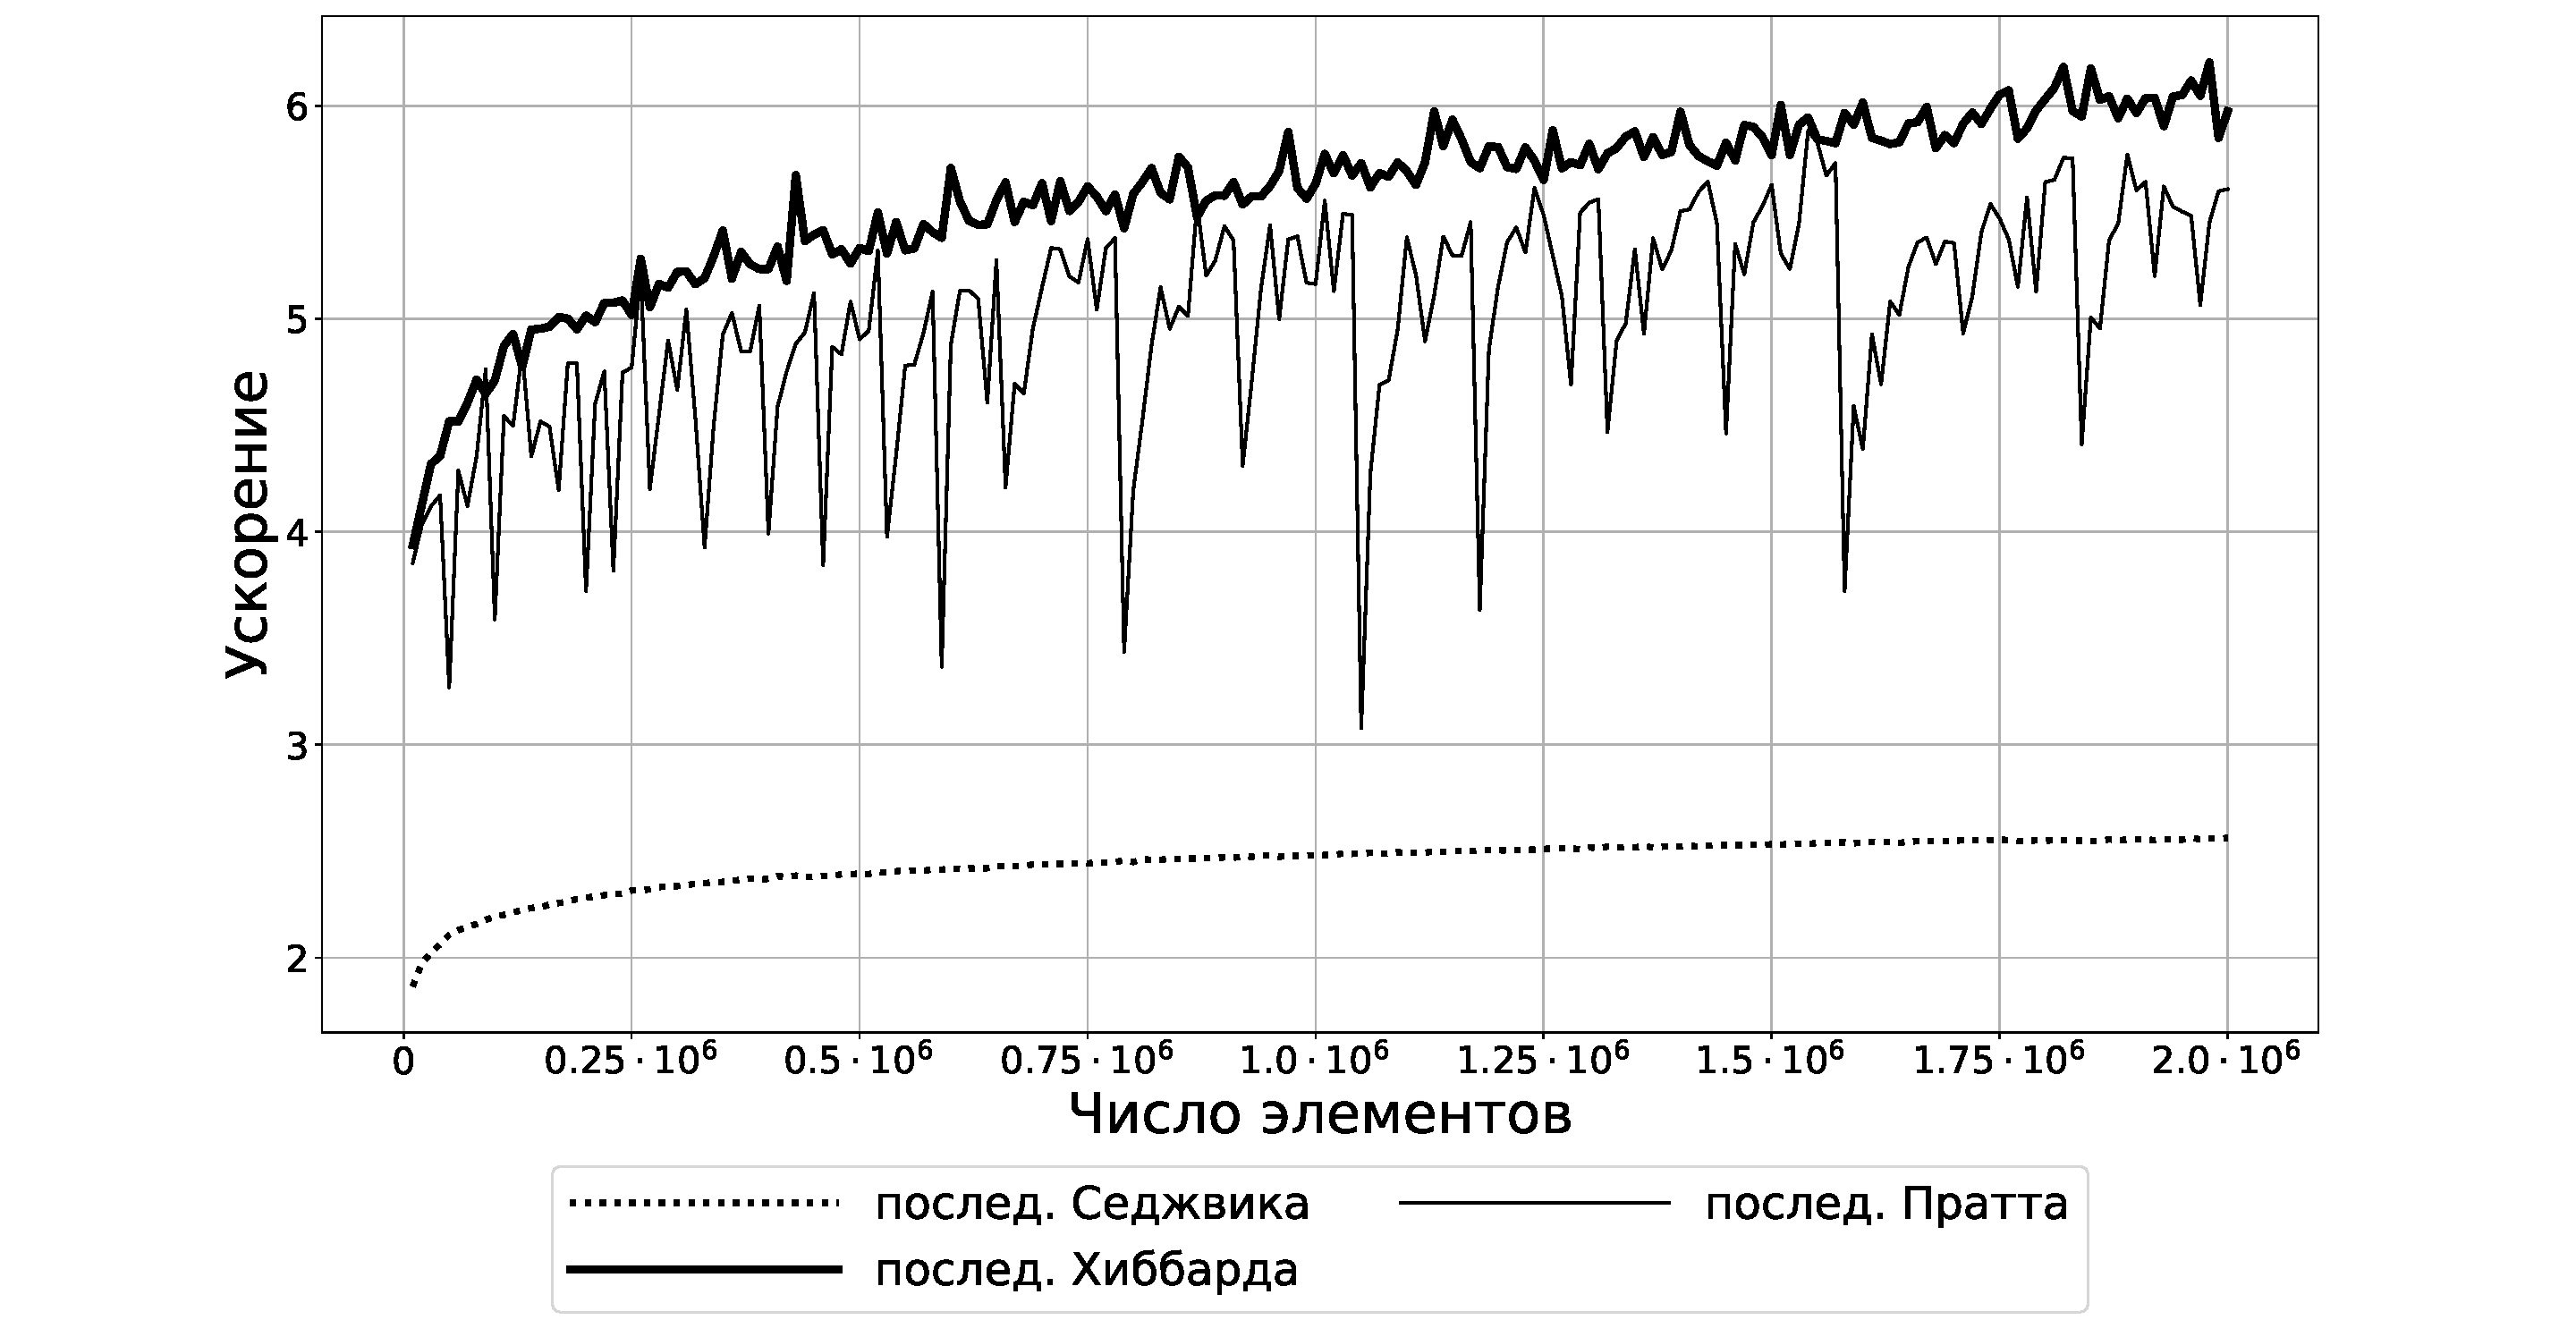
\includegraphics[width=10cm]{pics/theoretical_eff}
\caption{Сравнение теоретического ускорения векторизованной версии сортировки Шелла для различных последовательностей шагов}
\label{pic:acc_theor}
\end{figure}

\begin{figure}
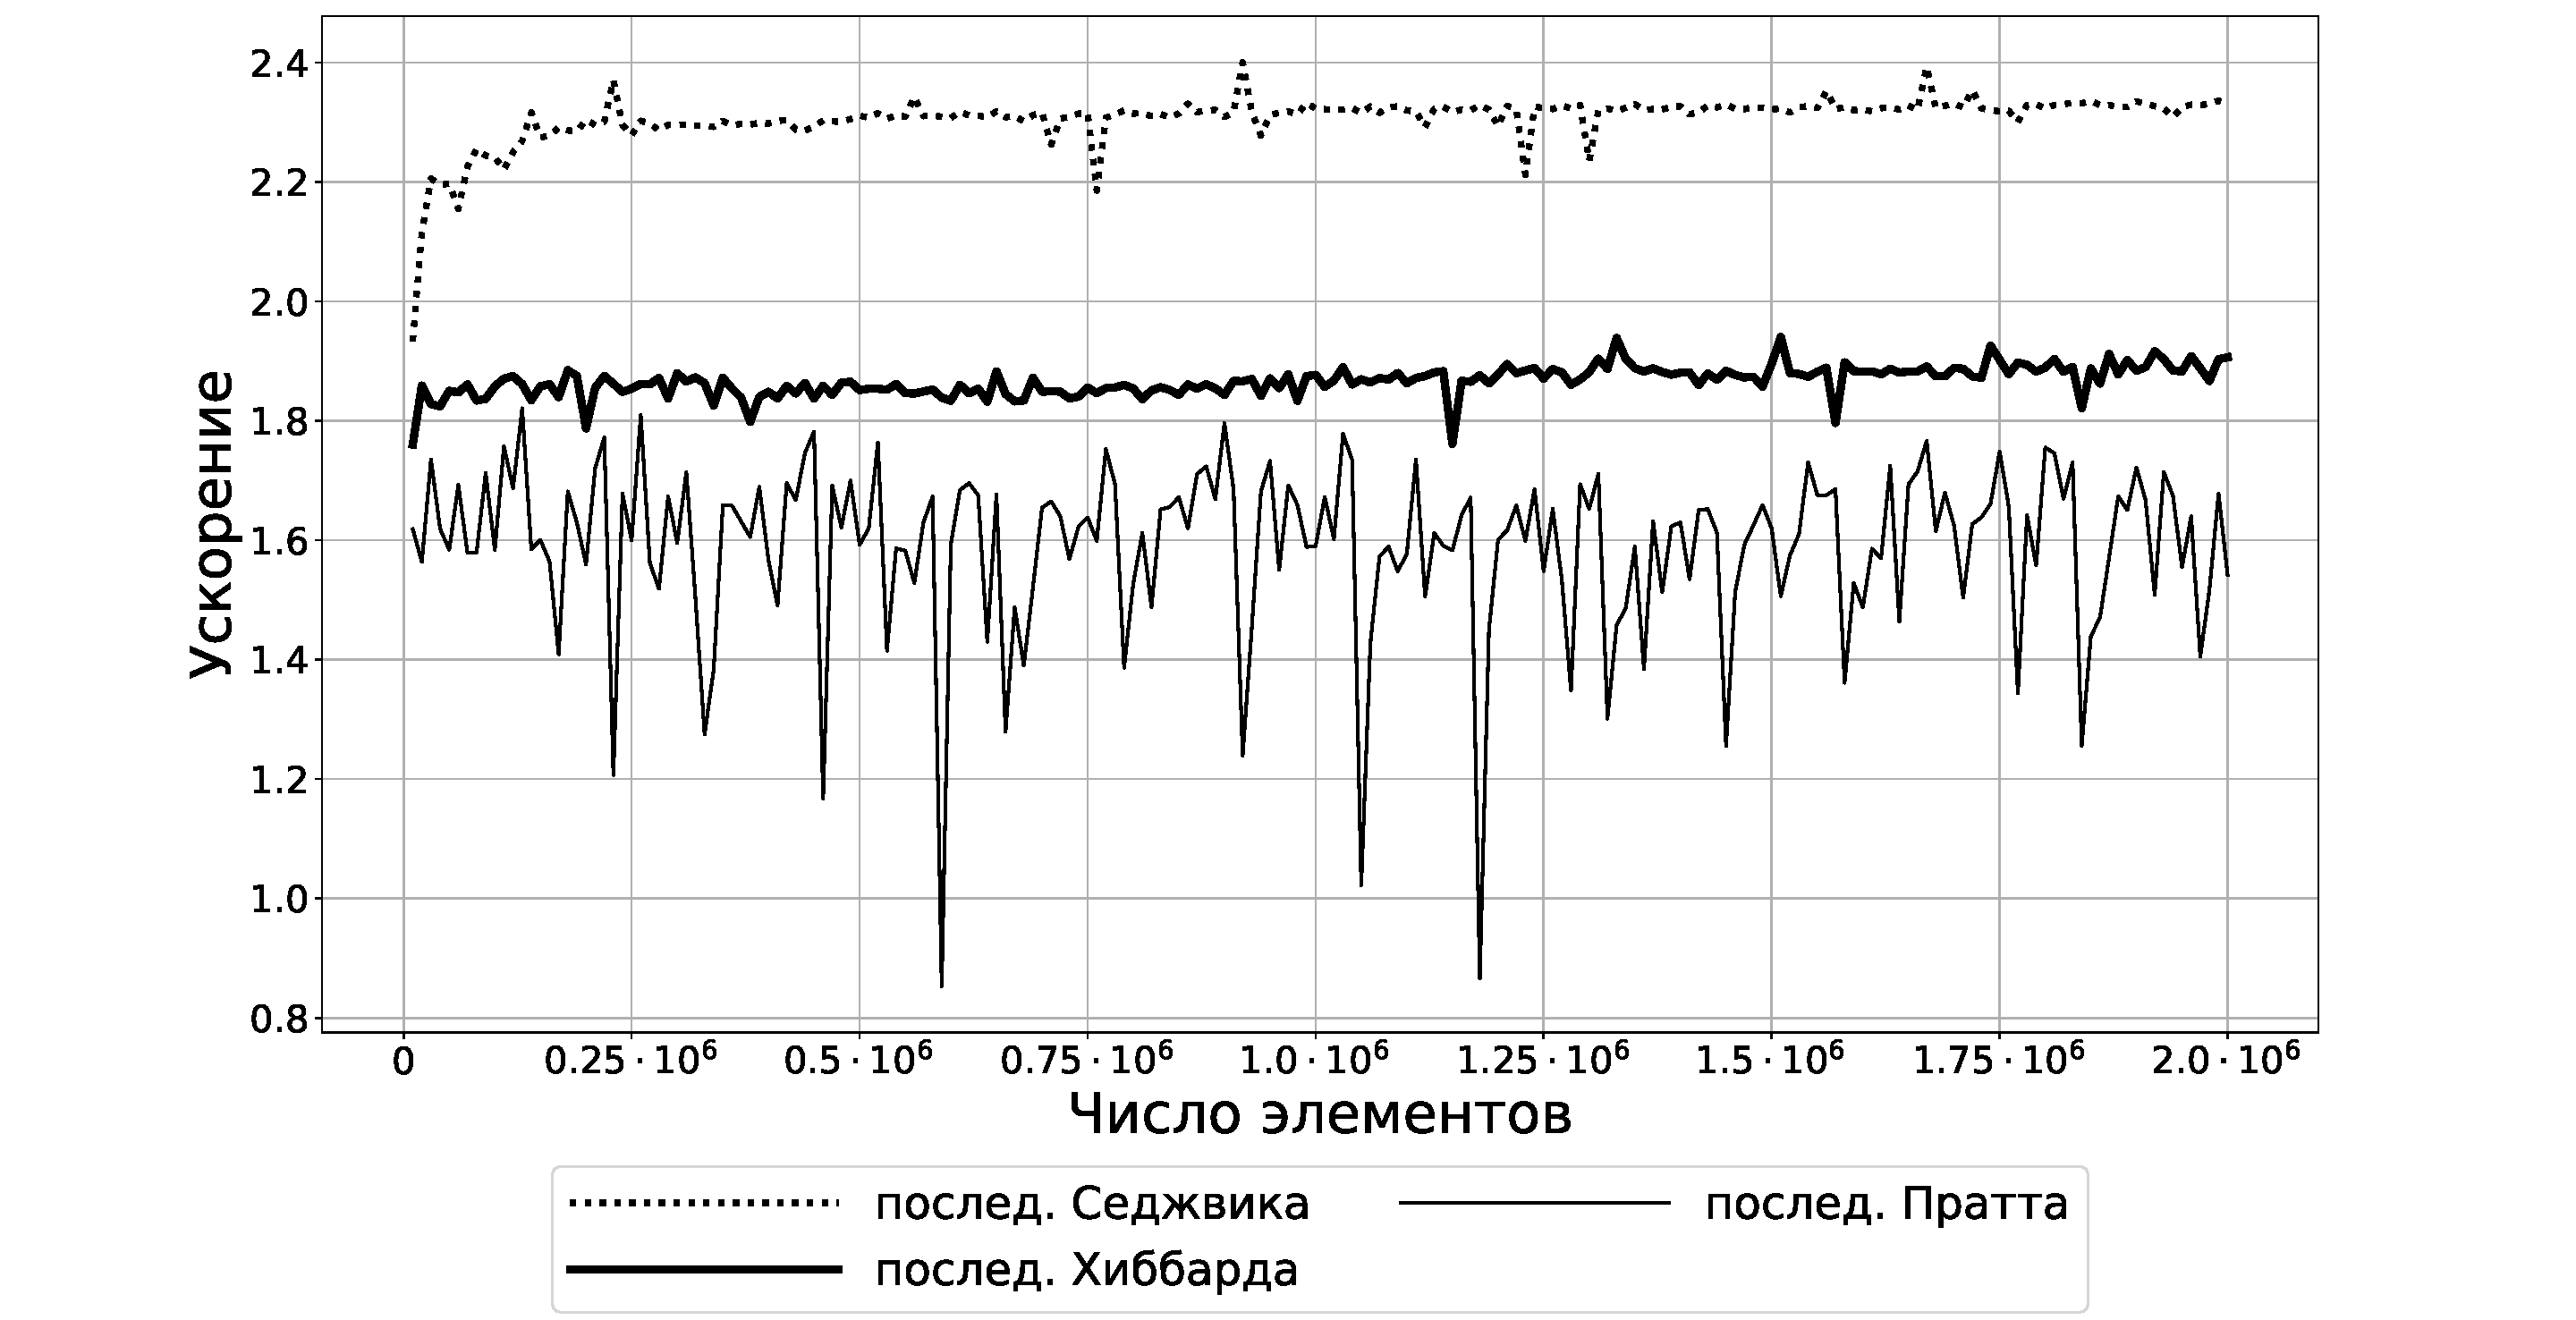
\includegraphics[width=10cm]{pics/experimental_eff}
\caption{Сравнение экспериментального ускорения векторизованной версии сортировки Шелла для различных последовательностей шагов}
\label{pic:acc_exp}
\end{figure}

Теоретическая оценка эффективности векторизации с использованием  последовательности Сэджвика оказалась ближе всего к экспериментальным результатам. Это может быть объяснено тем, что последовательность шагов $ks$ в данном случае достаточно короткая, и сортируемые срезы с разными значениями $k$ слабо коррелируют друг с другом.
В последовательности шагов Сэджвика присутствует только один шаг меньше 16 (это последний шаг $k = 1$), для всех остальных шагов доступно применение векторизации с максимальной плотностью.

\begin{figure}
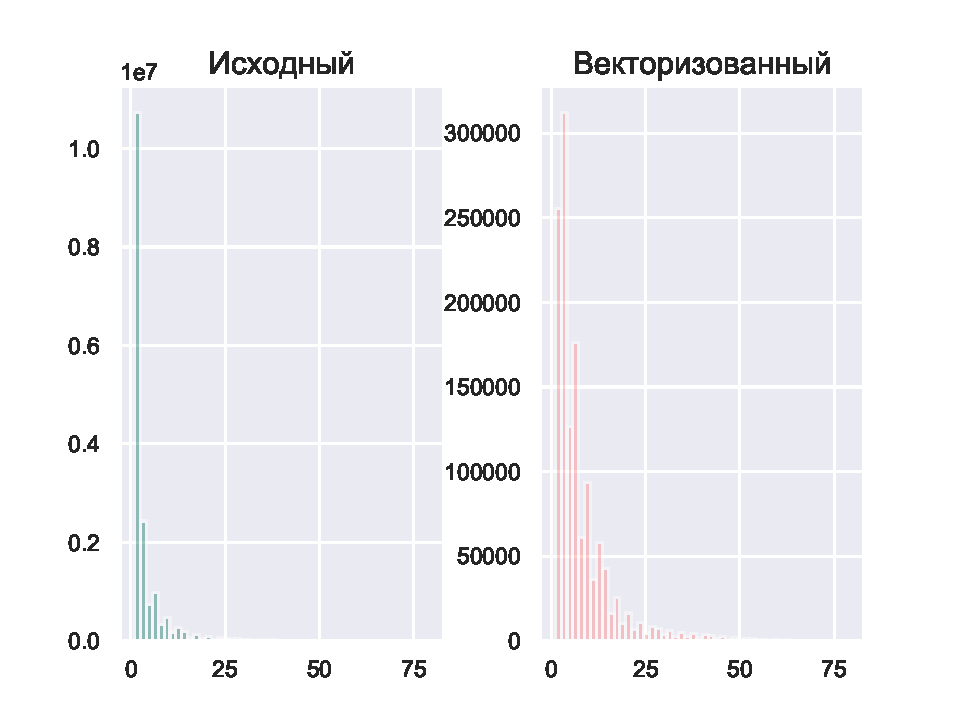
\includegraphics[width=8cm,height=6cm]{pics/pic_shell_k_4}
\caption{Гистограмма распределения количества итераций внутреннего цикла при сортировке с последовательностью Шелла при $k = 4$}
\label{pic:shell_k_4}
\end{figure}

\begin{figure}
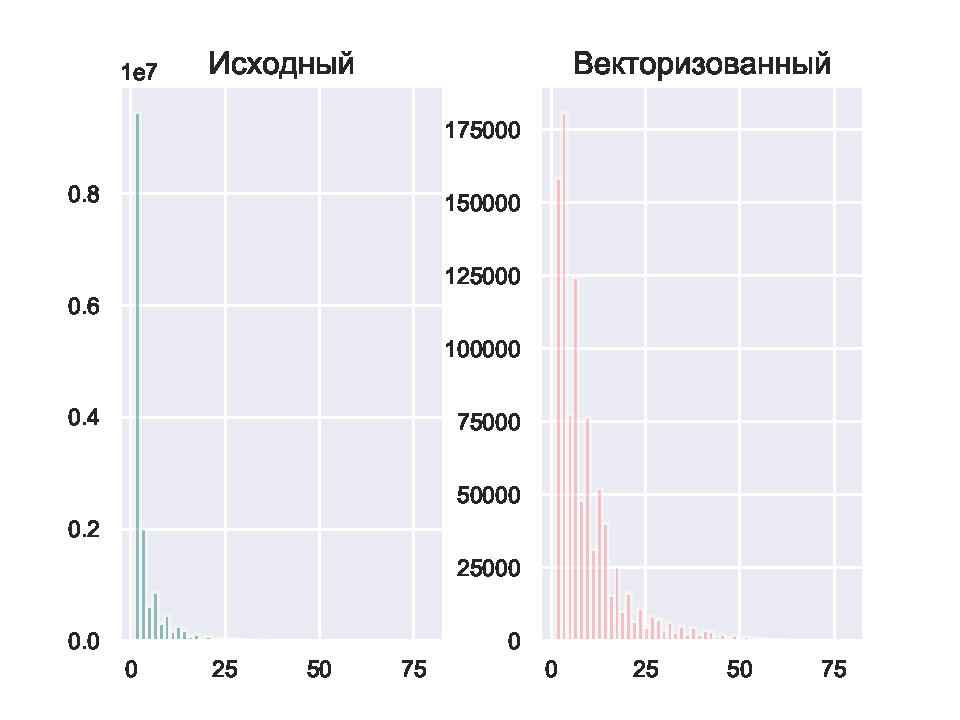
\includegraphics[width=8cm,height=6cm]{pics/pic_shell_k_15}
\caption{Гистограмма распределения количества итераций внутреннего цикла при сортировке с последовательностью Шелла при $k = 15$}
\label{pic:shell_k_15}
\end{figure}

\begin{figure}
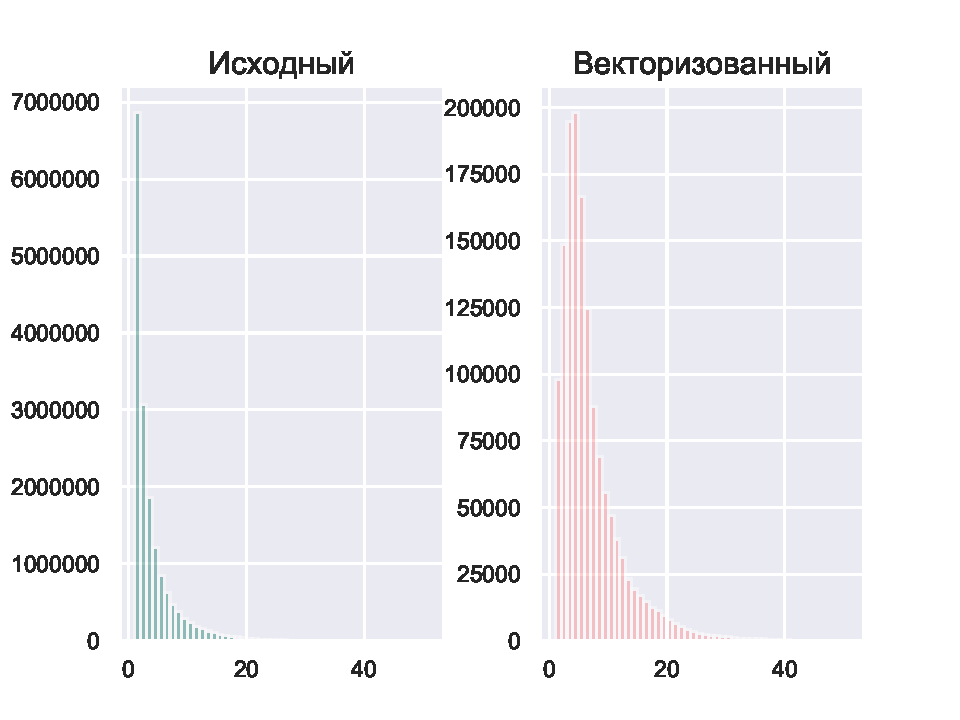
\includegraphics[width=8cm,height=6cm]{pics/pic_hibbard_k_3}
\caption{Гистограмма распределения количества итераций внутреннего цикла при сортировке с последовательностью Хиббарда при $k = 3$}
\label{pic:hibbard_k_3}
\end{figure}

\begin{figure}
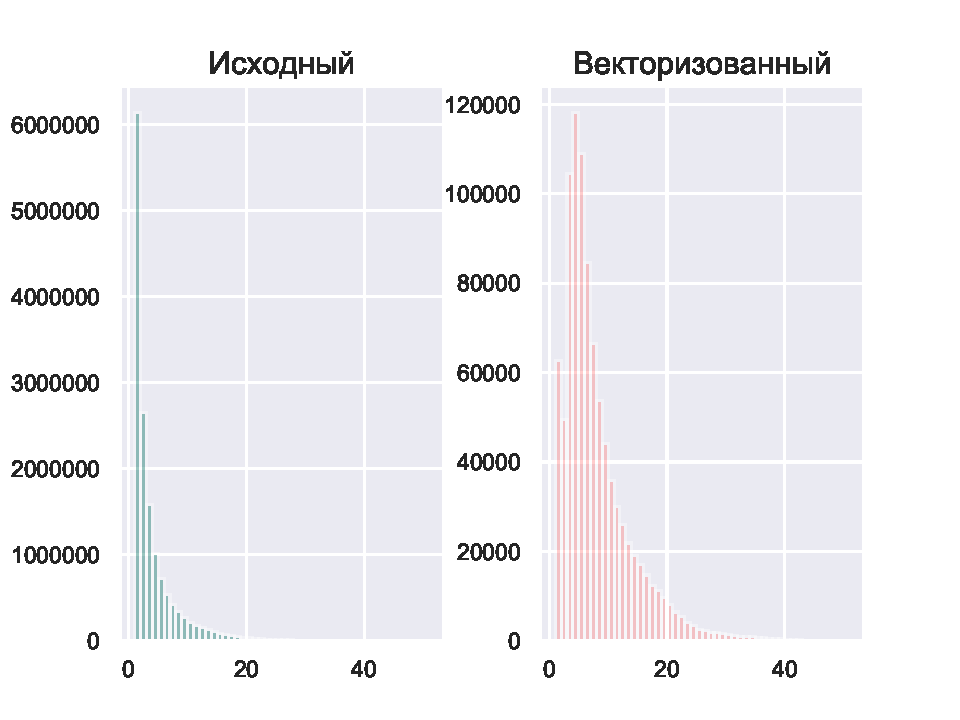
\includegraphics[width=8cm,height=6cm]{pics/pic_hibbard_k_15}
\caption{Гистограмма распределения количества итераций внутреннего цикла при сортировке с последовательностью Хиббарда при $k = 15$}
\label{pic:hibbard_k_15}
\end{figure}

Противоположностью последовательности Сэджвика является последовательность шагов Пратта, содержащая всевозможные шаги вида $2^i3^j$.
Во-первых, эта последовательность очень длинная и содержит сразу 8 значений, которые меньше максимальной ширины векторизации, что негативно сказывается на производительности.
Во-вторых, срезы, индуцированные такими шагами, являются принципиально сильно коррелирующими, это приводит к нерегулярному снижению количества итераций во внутреннем цикле невекторизованной версии.
В итоге мы имеем очень непостоянный график как теоретического, так и и экспериментального ускорения, с низкой эффективностью векторизации и резкими провалами, опускающимися даже ниже единицы.

\section*{Заключение}

На примере сортировки Шелла был рассмотрен крайне неудобный для векторизации контекст исполнения, представленный гнездом циклов с нерегулярным количеством итераций внутреннего цикла.
Даже теоретическое ускорение для такого контекста далеко от идеальной верхней границы, а на практике и вовсе может быть получен негативный эффект от применения векторизации.
Такие свойства характерны прежде всего для дискретных задач, к числу которых относятся задачи сортировки, комбинаторики и перечисления.
При использовании векторизации для таких задач характер их исполнения должен быть оценен отдельно в каждом конкретном случае для избежания неожиданной деградации эффективности программного кода.
\\


\textit{Работа выполнена в МСЦ РАН в рамках государственного задания по теме 0065-2019-0016 (reg. no. АААА-А19-119011590098-8). При проведении исследований использовался суперкомпьютер МВС-10П, находящийся в МСЦ РАН.}


\begin{thebibliography}{30}

\RBibitem{intel_manual}
\by
Intel 64 and IA-32 Architectures Software Developer's Manual. Combined volumes: 1, 2A, 2B, 2C, 2D, 3A, 3B, 3C, 3D and 4. Intel Corporation. 2017. URL: https://software.intel.com/en-us/download/intel-64-and-ia-32-architectures-sdm-combined-volumes-1-2a-2b-2c-2d-3a-3b-3c-3d-and-4 (дата обращения: 25.10.2018)

\Bibitem{Jeffers}
\by Jeffers James, Reinders James, Sodani Avinash 
\book Intel Xeon Phi processor high performance programming
\bookinfo Knights Landing Edition
\edition 2 ed.
\publ Morgan Kaufmann Publ.
\yr 2016
\totalpages 632

\RBibitem{compiler_guide}
\by
Intel C++ Compiler 16.0 User and Reference Guide. Intel Corporation. 2015. URL: https://software.intel.com/en-us/articles/intel-c-compiler-160-for-windows-release-notes-for-intel-parallel-studio-xe-2016 (дата обращения: 25.10.2018)

\RBibitem{intrinsic_guide}
\by
Intel Intrinsics Guide. URL: https://software.intel.com/sites/landingpage/
IntrinsicsGuide (дата обращения: 02.11.2018)

\RBibitem{Knuth}
\by Кнут Дональд
\book Искусство программирования
\bookvol 3
\voltitle Сортировка и поиск
\publ Вильямс
\publaddr М.
\yr 1994
\totalpages 832

\RBibitem{Volkonskyi}
\by Волконский В.Ю., Окунев С.К.
\paper Предикатное представление как основа оптимизации программы для архитектур с явно выраженной параллельностью
\jour Информационные технологии
\yr 2003
\issue 4
\pages 36--45

\RBibitem{Hib_seq}
\by
A168604, последовательность Хиббарда. URL: https://oeis.org/A168604 (дата обращения 02.11.18)

\RBibitem{Pratt_seq}
\by
A003586, последовательность Пратта. https://oeis.org/A003586 (дата обращения 02.11.18)

\RBibitem{Sedjw_seq}
\by
A033622, последовательность Седжвика. URL: https://oeis.org/A033622 (дата обращения 02.11.18)

% Ссылки для обзора.
% По степени релевантности.

\RBibitem{Bramas}
\by Bramas B.
\paper Fast Sorting Algorithms using AVX-512 on Intel Knights Landing
\jour International Journal of Advanced Computer Science and Applications
\yr 2017
\vol 8
\issue 10
\pages 337--344
\URL https://www.researchgate.net/publication/316542898_Fast_Sorting_Algorithms_using_AVX-512_on_Intel_Knights_Landing

\RBibitem{Dikarev}
\by Дикарев Н. И., Шабанов Б. М., Шмелев А. С.
\paper Выполнение задач сортировки на векторном процессоре с архитектурой управления потоком данных
\jour Программные системы: Теория и приложения
\yr 2017
\vol 8
\issue 4
\pages 305--317
\URL http://psta.psiras.ru/read/psta2017_4_305-317.pdf
\crossref{http://dx.doi.org/10.25209/2079-3316-2017-8-4-305-317}

\RBibitem{Guskova}
\by Гуськова М. С., Бараш Л. Ю., Щур Л. Н.
\paper Применение AVX512-векторизации для увеличения производительности генератора псевдослучайных чисел
\jour Труды ИСП РАН
\yr 2018
\vol 30
\issue 1
\pages 115--126

\RBibitem{Krzikalla}
\by O. Krzikalla, F. Wende, M. Hohnerbach
\paper Dynamic SIMD vector lane scheduling
\jour Lect. Notes Comput. Sci.
\yr 2016
\issue 9945
\pages 354-365

\RBibitem{Benderskij}
\by Бендерский Л. А., Рыбаков А. А., Шумилин С. С.
\paper Векторизация перемножения малоразмерных матриц специального вида с использованием инструкций AVX-512
\jour Современные информационные технологии и ИТ-образование
\yr 2018
\vol 14
\issue 3
\pages 594--602
\URL http://sitito.cs.msu.ru/index.php/SITITO/article/view/424
\crossref{http://dx.doi.org/10.25559/SITITO.14.201803.594-602}

\RBibitem{Zhang}
\by Zhang H., Rupp K., Mills R. T., Smith B. F.
\paper Vectorized Parallel Sparse Matrix-Vector Multiplication in PETSc Using AVX-512
\paperinfo ICPP 2018
\yt 2018
\crossref{http://dx.doi.org/10.1145/3225058.3225100}

\RBibitem{Sing}
\by Sing J. T. K., Sheikh U. U., Mokji M., Alias N. E.
\paper Hadamard Transform Improvement for HEVC using Intel AVX-512
\paperinfo 2019 IEEE 9th Simposium on Computer Applications & Industrial Electronics (ISCAIE)
\yr 2019
\crossref{http://dx.doi.org/10.1109/ISCAIE.2019.8743904}

\RBibitem{Kim}
\by Kim R., Choi J., Lee M.
\paper Optimizing parallel GEMM routines using auto-tuning with Intel AVX-512
\jour HPC ASIA
\yr 2019
\crossref{http://dx.doi.org/10.1145/3293320.3293334}

\RBibitem{Rybakov}
\by Рыбаков А. А., Шумилин С. С.
\paper Векторизация сильно разветвленного управления с помощью инструкций AVX-512
\your Труды НИИСИ РАН
\yr 2018
\vol 8
\issue 4
\pages 114--126
\URL https://www.niisi.ru/tr/2018_T8_N4.pdf
\crossref{http://dx.doi.org/10.25682/NIISI.2018.4.0014}

\RBibitem{Ginting}
\by Ginting B. M., Mundani R.-P.
\paper Comparison of Shallow Water Solvers: Application for Dam-Break and Tsunami Cases with Reordering Strategy for Efficient Vectorization on Modern Hardware
\your Water -- Open Access Journal
\yr 2019
\vol 11
\issue 639
\pages 1--31
\URL http://www.mdpi.com/journal/water
\crossref{http://dx.doi.org/10.3390/w11040639}

\end{thebibliography}
\end{document}

